\begin{figure*}[!hbt]
  \centering
  \subfigure{
    \label{fig:temporal-batch4--runtime}
    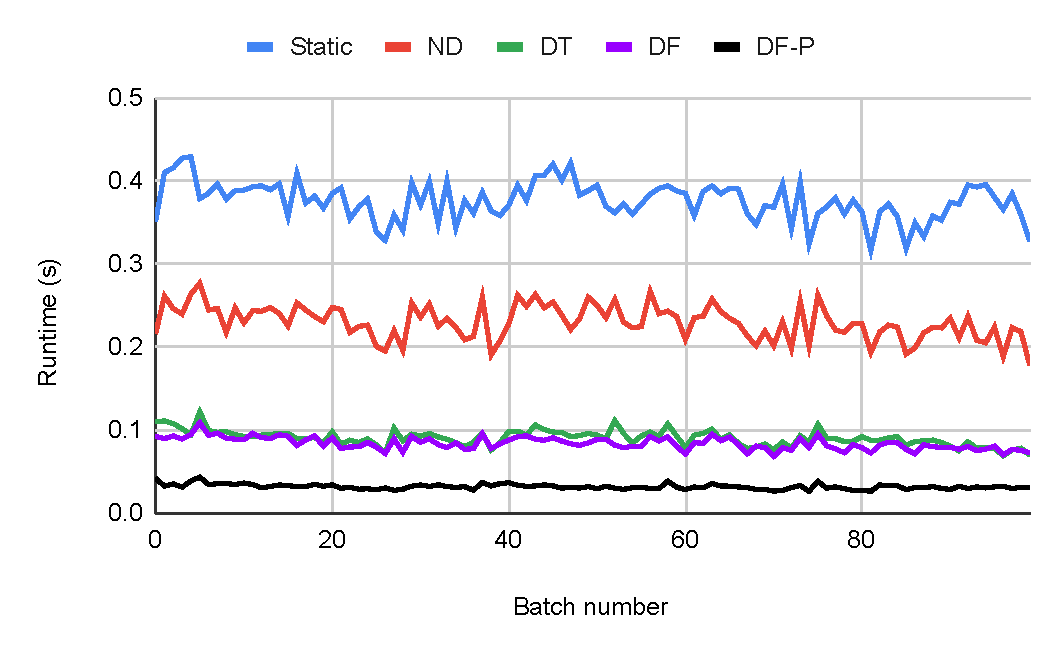
\includegraphics[width=0.48\linewidth]{out/temporal-batch4-runtime.pdf}
  }
  \subfigure{
    \label{fig:temporal-batch4--error}
    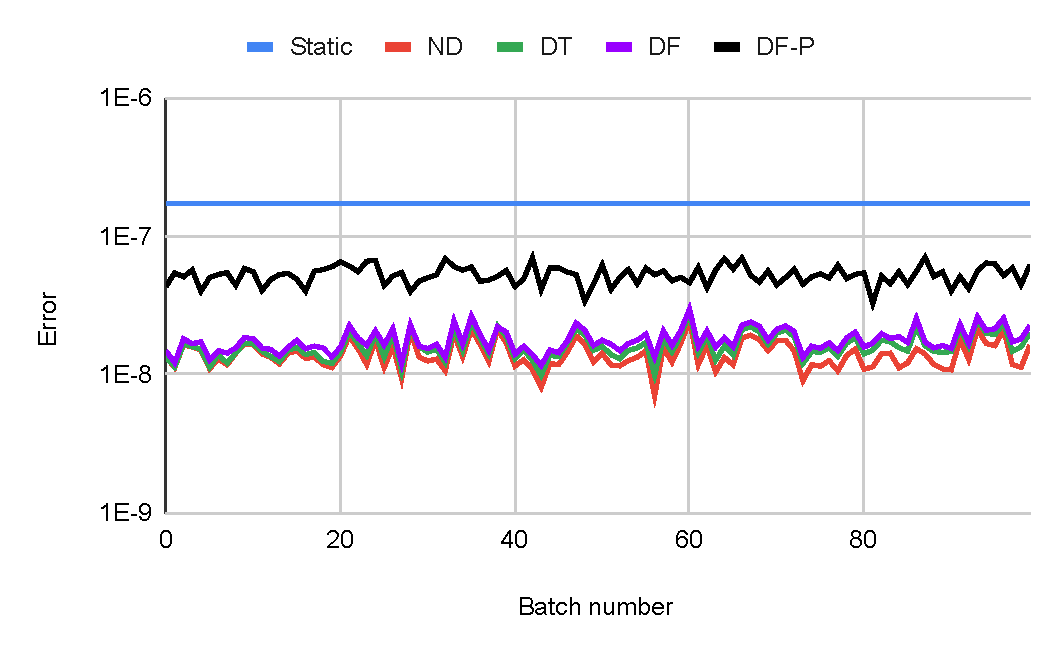
\includegraphics[width=0.48\linewidth]{out/temporal-batch4-error.pdf}
  } \\[-2ex]
  \caption{Average Relative runtime with asynchronous implementations of \textit{Static}, \textit{Naive-dynamic}, \textit{Dynamic Traversal}, and \textit{Dynamic Frontier} approach compared to their respective synchronous implementations, on batch updates of size $10^{-7}|E|$ to $0.1|E|$ (right), and overall (left). The results indicate that asynchronous implementations are faster than synchronous ones, especially for smaller batch sizes. This is due to a somewhat faster convergence and the absence of copy overhead (for \textit{Dynamic Traversal} and \textit{Dynamic Frontier} approaches).}
  \label{fig:temporal-batch4}
\end{figure*}
